%%%%%%%%%%%%%%%%%%%%%%%%%%%%%%%%%%%%%%%%%%%%%%%%%%%%%%%%%%%%%%%%%%%%%%%%%%%%%%%%
%2345678901234567890123456789012345678901234567890123456789012345678901234567890
%        1         2         3         4         5         6         7         8
%% PP_Report.tex
%% V1.4
%% 2015/11/30
%% by Rui Santos Cruz
%% This is a skeleton file using PPIEEEtran.cls
%% (requires PPIEEEtran.cls) 
% !TEX root = ./main.tex
%%%%%%%%%%%%%%%%%%%%%%%%%%%%%%%%%%%%%%%%%%%%%%%%%%%%%%%%%%%%%%%%%%%%%%%%%%%%%%%%
\documentclass[a4paper,12pt,journal,twoside,compsoc]{PPIEEEtran}

% -----------------------------------------------------------------------------
% The Preamble document contains all the necessary Packages for typesetting
% Modify it to suit your needs
% -----------------------------------------------------------------------------
%%%%%%%%%%%%%%%%%%%%%%%%%%%%%%%%%%%%%%%%%%%%%%%%%%%%%%%%%%%%%%%%%%%%%%%%%%%%%%%%
%2345678901234567890123456789012345678901234567890123456789012345678901234567890
%        1         2         3         4         5         6         7         8
% Required Packages and commands
% --> Please Choose the MAIN LANGUAGE for the document in package BABEL (below)
% --> Please Choose the TYPE OF REPORT for the document in \ReportType (below)
% !TEX root = ./main.tex
% PP_Report_Preamble.tex
% V1.4
% 2015/11/30
% by Rui Santos Cruz
%%%%%%%%%%%%%%%%%%%%%%%%%%%%%%%%%%%%%%%%%%%%%%%%%%%%%%%%%%%%%%%%%%%%%%%%%%%%%%%%
%
% *** INPUT LANGUAGE PACKAGES ***

\usepackage[main=english]{babel}
\usepackage[utf8]{inputenc}
\usepackage{iflang}

% *** DEFINE THE TYPE OF REPORT ***
\newcommand*{\ReportType}{learning}% Uncomment line for Learning Report
%\newcommand*{\ReportType}{activity}% Uncomment line for Activity Report

% *** ACRONYM PACKAGES ***
% Put definition of Acronyms at the end of the document
\usepackage[printonlyused,nolist]{acronym}

% *** CITATION PACKAGES ***
\usepackage{cite}

% *** GRAPHICS RELATED PACKAGES ***
\usepackage[pdftex]{graphicx}
\DeclareGraphicsExtensions{.pdf,.jpeg,.png}

% *** MATH PACKAGES ***
\usepackage[cmex10]{amsmath}

% *** SPECIALIZED LIST PACKAGES ***
\usepackage{algorithmic}

% *** ALIGNMENT PACKAGES ***
\usepackage{array}

% *** SUBFIGURE PACKAGES ***
\usepackage[caption=false,font=normalsize,labelfont=sf,textfont=sf]{subfig}

% *** FLOAT PACKAGES ***
\usepackage{fixltx2e}

% *** PDF, URL AND HYPERLINK PACKAGES ***
\usepackage{url}

% *** BACKGROUND Material ***
\usepackage{eso-pic}
\usepackage[
  contents={},
  opacity=1,
  scale=1,
  color=blue!90
  ]{background}
  
% *** CONDITIONALS ***
\usepackage{ifthen}

% DEFINE COMMAND FOR: Report Type depending on language
\newcommand{\tlangRepActivity}{\IfLanguageName{english}{Activity Report}{Relatório de Atividade}}
\newcommand{\tlangRepLearning}{\IfLanguageName{english}{Learnings Report}{Relatório de Aprendizagens}}
%%%%%%%%%%%%%%%%%%%%%%%%%%%%%%%%%%%%%%%%%%%%%%%%%%%%%%%%%%%%%%%%%%%%%%%%%%%%%%%%
% DEFINE COMMAND FOR: Report Scoring Table Type
\newcommand{\lrScore}%
{\setlength{\unitlength}{1mm}{% % selecting unit length 
\fontfamily{phv}\selectfont
\begin{picture}(171.6,20) % picture environment with the size (dimensions)
% 32 length units wide, and 15 units high.
\setlength\fboxsep{0pt}
% Left Set with grading Scores
\put(0,0){\fcolorbox{gray}{gray!20}{%
          \framebox(15,4)[l]{\scriptsize{0.2-Weak}}}}
\put(0,4){\fcolorbox{gray}{gray!20}{%
          \framebox(15,4)[l]{\scriptsize{0.4-Fair}}}}
\put(0,8){\fcolorbox{gray}{gray!20}{%
          \framebox(15,4)[l]{\scriptsize{0.6-Good}}}}
\put(0,12){\fcolorbox{gray}{gray!20}{%
           \framebox(15,4)[l]{\scriptsize{0.8-V.Good}}}}
\put(0,16){\fcolorbox{gray}{gray!20}{%
           \framebox(15,4)[l]{\scriptsize{1.0-Excel}}}}
% Left+1 Set with Learning Rubrics
\put(16,0){\fcolorbox{cyan}{white}{%
          \framebox(12,12)[c]{\footnotesize{ }}}}
\put(28,0){\fcolorbox{cyan}{white}{%
          \framebox(12,12)[c]{\footnotesize{ }}}}          
\put(40,0){\fcolorbox{cyan}{white}{%
          \framebox(12,12)[c]{\footnotesize{ }}}}
\put(52,0){\fcolorbox{cyan}{white}{%
          \framebox(12,12)[c]{\footnotesize{ }}}}
\put(64,0){\fcolorbox{cyan}{white}{%
          \framebox(12,12)[c]{\footnotesize{ }}}}
\put(16,12){\fcolorbox{cyan}{white}{%
          \framebox(12,4)[c]{\tiny{Intro$\times 2$}}}}
\put(28,12){\fcolorbox{cyan}{white}{%
          \framebox(12,4)[c]{\tiny{Motiv$\times 2$}}}}          
\put(40,12){\fcolorbox{cyan}{white}{%
          \framebox(12,4)[c]{\tiny{Skills$\times 6$}}}}
\put(52,12){\fcolorbox{cyan}{white}{%
          \framebox(12,4)[c]{\tiny{Reflect$\times 6$}}}}
\put(64,12){\fcolorbox{cyan}{white}{%
          \framebox(12,4)[c]{\tiny{Sugg$\times 2$}}}}
\put(16,16){\fcolorbox{cyan}{cyan!20}{%
          \framebox(60,4)[c]{\footnotesize{LEARNINGS}}}}
% Middle Set with Document Rubrics
\put(77,0){\fcolorbox{green}{white}{%
          \framebox(12,12)[c]{\footnotesize{ }}}}
\put(89,0){\fcolorbox{green}{white}{%
          \framebox(12,12)[c]{\footnotesize{ }}}}
\put(101,0){\fcolorbox{green}{white}{%
          \framebox(12,12)[c]{\footnotesize{ }}}}
\put(113,0){\fcolorbox{green}{white}{%
          \framebox(12,12)[c]{\footnotesize{ }}}}
\put(125,0){\fcolorbox{green}{white}{%
          \framebox(12,12)[c]{\footnotesize{ }}}}
\put(137,0){\fcolorbox{green}{white}{%
          \framebox(12,12)[c]{\footnotesize{ }}}}
\put(77,12){\fcolorbox{green}{white}{%
          \framebox(12,4)[c]{\tiny{Struct $\times .25$}}}}
\put(89,12){\fcolorbox{green}{white}{%
          \framebox(12,4)[c]{\tiny{Ortog$\times .25$}}}}          
\put(101,12){\fcolorbox{green}{white}{%
          \framebox(12,4)[c]{\tiny{Gram$\times .25$}}}}
\put(113,12){\fcolorbox{green}{white}{%
          \framebox(12,4)[c]{\tiny{Form $\times .25$}}}}
\put(125,12){\fcolorbox{green}{white}{%
          \framebox(12,4)[c]{\tiny{Abstr $\times .5$}}}}
\put(137,12){\fcolorbox{green}{white}{%
          \framebox(12,4)[c]{\tiny{Concl $\times .5$}}}}
\put(77,16){\fcolorbox{green}{green!20}{%
          \framebox(72,4)[c]{\footnotesize{DOCUMENT}}}}
% Right Set with Penalties
\put(150,0){\fcolorbox{red}{white}{%
          \framebox(10,12)[c]{\footnotesize{ }}}}
\put(160,0){\fcolorbox{red}{white}{%
          \framebox(10,12)[c]{\footnotesize{ }}}}
\put(170,0){\fcolorbox{red}{white}{%
          \framebox(10,12)[c]{\footnotesize{ }}}}
\put(150,12){\fcolorbox{red}{white}{%
          \framebox(10,4)[c]{\tiny{Titles $\times .5$}}}}
\put(160,12){\fcolorbox{red}{white}{%
          \framebox(10,4)[c]{\tiny{Files $\times .5$}}}}
\put(170,12){\fcolorbox{red}{white}{%
          \framebox(10,4)[c]{\tiny{IDs $\times .5$}}}}
\put(150,16){\fcolorbox{red}{red!20}{%
          \framebox(30,4)[c]{\footnotesize{PENALTY}}}}
\end{picture}
}}
%%%%%%%%%%%%%%%%%%%%%%%%%%%%%%%%%%%%%%%%%%%%%%%%%%%%%%%%%%%%%%%%%%%%%%%%%%%%%%%%
%\newcommand{\arScore}%
\newcommand{\arScore}%
{\setlength{\unitlength}{1mm}{% % selecting unit length 
\fontfamily{phv}\selectfont
\begin{picture}(171.6,20) % picture environment with the size (dimensions)
% 32 length units wide, and 15 units high.
\setlength\fboxsep{0pt}
% Left Set with grading Scores
\put(0,0){\fcolorbox{gray}{gray!20}{%
          \framebox(15,4)[l]{\scriptsize{0.2-Weak}}}}
\put(0,4){\fcolorbox{gray}{gray!20}{%
          \framebox(15,4)[l]{\scriptsize{0.4-Fair}}}}
\put(0,8){\fcolorbox{gray}{gray!20}{%
          \framebox(15,4)[l]{\scriptsize{0.6-Good}}}}
\put(0,12){\fcolorbox{gray}{gray!20}{%
           \framebox(15,4)[l]{\scriptsize{0.8-V.Good}}}}
\put(0,16){\fcolorbox{gray}{gray!20}{%
           \framebox(15,4)[l]{\scriptsize{1.0-Excel}}}}
% Left+1 Set with Activity Rubrics
\put(16,0){\fcolorbox{yellow}{white}{%
          \framebox(12,12)[c]{\footnotesize{ }}}}
\put(28,0){\fcolorbox{yellow}{white}{%
          \framebox(12,12)[c]{\footnotesize{ }}}}          
\put(40,0){\fcolorbox{yellow}{white}{%
          \framebox(12,12)[c]{\footnotesize{ }}}}
\put(52,0){\fcolorbox{yellow}{white}{%
          \framebox(12,12)[c]{\footnotesize{ }}}}
\put(64,0){\fcolorbox{yellow}{white}{%
          \framebox(12,12)[c]{\footnotesize{ }}}}
\put(16,12){\fcolorbox{yellow}{white}{%
          \framebox(12,4)[c]{\tiny{Intro$\times 2$}}}}
\put(28,12){\fcolorbox{yellow}{white}{%
          \framebox(12,4)[c]{\tiny{Object$\times 2$}}}}          
\put(40,12){\fcolorbox{yellow}{white}{%
          \framebox(12,4)[c]{\tiny{Plan$\times 4$}}}}
\put(52,12){\fcolorbox{yellow}{white}{%
          \framebox(12,4)[c]{\tiny{Exec$\times 6$}}}}
\put(64,12){\fcolorbox{yellow}{white}{%
          \framebox(12,4)[c]{\tiny{Result$\times 4$}}}}
\put(16,16){\fcolorbox{yellow}{yellow!20}{%
          \framebox(60,4)[c]{\footnotesize{ACTIVITY}}}}
% Middle Set with Document Rubrics
\put(77,0){\fcolorbox{green}{white}{%
          \framebox(12,12)[c]{\footnotesize{ }}}}
\put(89,0){\fcolorbox{green}{white}{%
          \framebox(12,12)[c]{\footnotesize{ }}}}
\put(101,0){\fcolorbox{green}{white}{%
          \framebox(12,12)[c]{\footnotesize{ }}}}
\put(113,0){\fcolorbox{green}{white}{%
          \framebox(12,12)[c]{\footnotesize{ }}}}
\put(125,0){\fcolorbox{green}{white}{%
          \framebox(12,12)[c]{\footnotesize{ }}}}
\put(137,0){\fcolorbox{green}{white}{%
          \framebox(12,12)[c]{\footnotesize{ }}}}
\put(77,12){\fcolorbox{green}{white}{%
          \framebox(12,4)[c]{\tiny{Struct $\times .25$}}}}
\put(89,12){\fcolorbox{green}{white}{%
          \framebox(12,4)[c]{\tiny{Ortog$\times .25$}}}}          
\put(101,12){\fcolorbox{green}{white}{%
          \framebox(12,4)[c]{\tiny{Gram$\times .25$}}}}
\put(113,12){\fcolorbox{green}{white}{%
          \framebox(12,4)[c]{\tiny{Form $\times .25$}}}}
\put(125,12){\fcolorbox{green}{white}{%
          \framebox(12,4)[c]{\tiny{Abstr $\times .5$}}}}
\put(137,12){\fcolorbox{green}{white}{%
          \framebox(12,4)[c]{\tiny{Concl $\times .5$}}}}
\put(77,16){\fcolorbox{green}{green!20}{%
          \framebox(72,4)[c]{\footnotesize{DOCUMENT}}}}
% Right Set with Penalties
\put(150,0){\fcolorbox{red}{white}{%
          \framebox(10,12)[c]{\footnotesize{ }}}}
\put(160,0){\fcolorbox{red}{white}{%
          \framebox(10,12)[c]{\footnotesize{ }}}}
\put(170,0){\fcolorbox{red}{white}{%
          \framebox(10,12)[c]{\footnotesize{ }}}}
\put(150,12){\fcolorbox{red}{white}{%
          \framebox(10,4)[c]{\tiny{Titles $\times .5$}}}}
\put(160,12){\fcolorbox{red}{white}{%
          \framebox(10,4)[c]{\tiny{Files $\times .5$}}}}
\put(170,12){\fcolorbox{red}{white}{%
          \framebox(10,4)[c]{\tiny{IDs $\times .5$}}}}
\put(150,16){\fcolorbox{red}{red!20}{%
          \framebox(30,4)[c]{\footnotesize{PENALTY}}}}
\end{picture}
}}

% DEFINE COMMAND FOR: Printing Scoring Table Type
\newcommand\BackgroundPic{%
\put(-15,12){%
\parbox[b][\paperheight]{\paperwidth}{%
\vfill
\centering
\ifthenelse{\equal{\ReportType}{activity}}{\arScore}{\lrScore}}}}
% Printing the Scoring Table
\AddToShipoutPicture*{\BackgroundPic}

% Print Vertical Identifications on even and odd pages
\AddEverypageHook{%
  \ifthenelse{\isodd{\value{page}}}%
  {\backgroundsetup{
    angle=90,
    position={-0.1\textwidth,-1.055\textheight},
    contents={\tiny{PP-2015 V1.4}}
    }% Odd Pages
  }%
  {\backgroundsetup{
    angle=90,
    position={0.97\textwidth,-1.05\textheight},%
    contents={\ifthenelse{\equal{\ReportType}{activity}}{%
              \tiny{\tlangRepActivity}}{\tiny{\tlangRepLearning}}}
    }% Even Pages
  }%
  \BgMaterial}
% correct bad hyphenation here
\hyphenation{op-tical net-works semi-conduc-tor}
%%%%%%%%%%%%%%%%%%%%%%%%%%%%%%%%%%%%%%%%%%%%%%%%%%%%%%%%%%%%%%%%%%%%%%%%%%%%%%%%
%2345678901234567890123456789012345678901234567890123456789012345678901234567890
%        1         2         3         4         5         6         7         8
\begin{document}
%%%%%%%%%%%%%%%%%%%%%%%%%%%%%%%%%%%%%%%%%%%%%%%%%%%%%%%%%%%%%%%%%%%%%%%%%%%%%%%%
%2345678901234567890123456789012345678901234567890123456789012345678901234567890
%        1         2         3         4         5         6         7         8
%% PP_Report_Cover.tex
%% V1.4
%% 2015/11/30
%% by Rui Santos Cruz
% !TEX root = ./main.tex
%%%%%%%%%%%%%%%%%%%%%%%%%%%%%%%%%%%%%%%%%%%%%%%%%%%%%%%%%%%%%%%%%%%%%%%%%%%%%%%%
% paper title
% can use linebreaks \\ within to get better formatting as desired
% Do not put math or special symbols in the title.
\title{Por2folios Platform}
%%%%%%%%%%%%%%%%%%%%%%%%%%%%%%%%%%%%%%%%%%%%%%%%%%%%%%%%%%%%%%%%%%%%%%%%%%%%%%%%
% Author names
%
% note positions of commas and nonbreaking spaces ( ~ ) LaTeX will not break
% a structure at a ~ so this keeps an author's name from being broken across
% two lines.
% use \thanks{} to gain access to the first footnote area
% a separate \thanks must be used for each paragraph.
%
%\IEEEcompsocitemizethanks is a special \thanks that produces the bulleted
% lists for "first footnote" author affiliations. 
% Use \IEEEcompsocthanksitem which works much like \item
% for each affiliation group.
\author{Francisco~Maria~Calisto% <-this % stops a space
% Change the Course Name 
% note: need leading \protect in front of \\ to get a newline within \thanks as
% \\ is fragile and will error, could use \hfil\break instead.
\IEEEcompsocitemizethanks{
\IEEEcompsocthanksitem Bruno~Cardoso, nr. 72619,\protect\\ 
E-mail: bruno.f.cardoso@tecnico.ulisboa.pt,
\IEEEcompsocthanksitem Francisco~Maria~Calisto, nr. 70916,\protect\\
E-mail: francisco.calisto@tecnico.ulisboa.pt,
\IEEEcompsocthanksitem Nuno~Sousa, nr. 73216,\protect\\
E-mail: nuno.g.sousa@tecnico.ulisboa.pt,\protect\\
Instituto Superior Técnico, Universidade de Lisboa.\protect\\}% <-this % stops an unwanted space}% <-this % stops an unwanted space
\thanks{Manuscrito recebido em Julho 24, 2016.}
}
%%%%%%%%%%%%%%%%%%%%%%%%%%%%%%%%%%%%%%%%%%%%%%%%%%%%%%%%%%%%%%%%%%%%%%%%%%%%%%%%
% The paper headers
\markboth{Por2folios}%
% for a single student
%{Surname}% : for a single student 
% for a Group Report 
{Surname \MakeLowercase{\textit{et al.}}}% : for a Group Report 
%
% The only time the second header will appear is for the odd numbered pages
% after the title page when using the twoside option.
%%%%%%%%%%%%%%%%%%%%%%%%%%%%%%%%%%%%%%%%%%%%%%%%%%%%%%%%%%%%%%%%%%%%%%%%%%%%%%%%
% Prints in Subtitle the type of Report
% PLEASE DO NOT CHANGE THIS SECTION
\IEEEspecialpapernotice{%
\ifthenelse{\equal{\ReportType}{activity}}{%
\tlangRepActivity}{\tlangRepLearning}
}
%%%%%%%%%%%%%%%%%%%%%%%%%%%%%%%%%%%%%%%%%%%%%%%%%%%%%%%%%%%%%%%%%%%%%%%%%%%%%%%%

\acrodef{VM}{Virtual Machine}
\acrodef{CMS}{Content Management Systems}
\acrodef{CPU}{Central Processing Unit}
\acrodef{GUI}{Graphical User Interface}
\acrodef{HTTP}{Hypertext Transfer Protocol}
\acrodef{IST}{Instituto Superior Técnico}	
\acrodef{INESC}{Instituto de Egenharia de Sistemas e Computadores}
\acrodef{PC}{Personal Computer}
%%%%%%%%%%%%%%%%%%%%%%%%%%%%%%%%%%%%%%%%%%%%%%%%%%%%%%%%%%%%%%%%%%%%%%%%%%%%%%%%
% The paper Abstract and Keywords
\IEEEtitleabstractindextext{%
\begin{abstract}
This report describes my experience with the development of the Por2Folios platform. It describes how I was introduced to the platform, how I was integrated in the development team and what I contributed to the platform. It contains some thoughts on what I learned with the experience and how it will affect me as a person. It also tries to give some insight on what to expect with the continued platform development in the future.
\end{abstract}
%
\begin{IEEEkeywords}
Por2Folios, Learning Report, WordPress, Portfolio.
\end{IEEEkeywords}}
%%%%%%%%%%%%%%%%%%%%%%%%%%%%%%%%%%%%%%%%%%%%%%%%%%%%%%%%%%%%%%%%%%%%%%%%%%%%%%%%
% make the title area
\maketitle

\IEEEdisplaynontitleabstractindextext
\IEEEpeerreviewmaketitle
%%%%%%%%%%%%%%%%%%%%%%%%%%%%%%%%%%%%%%%%%%%%%%%%%%%%%%%%%%%%%%%%%%%%%%%%%%%%%%%%
%%%%%%%%%%%%%%%%%%%%%%%%%%%%%%%%%%%%%%%%%%%%%%%%%%%%%%%%%%%%%%%%%%%%%%%%%%%%%%%%
\section{Introduction}
% The very first letter is a 2 line initial drop letter followed
% by the rest of the first word in caps (small caps for compsoc).
% 
% form to use if the first word consists of a single letter:
% \IEEEPARstart{A}{demo} file is ....
% 
% Here we have the typical use of a "E" for an initial drop letter
% and "STE" in caps to complete the first word.
\IEEEPARstart{I}{n} this report I will describe my experiences while developing the Por2Folios platform. This was made as an activity for the portfolio IV course. This course tries to give students an opportunity to develop their \textit{soft-skills}. In order to do so, students choose from a plethora of activities that are presented and complete it during the semester.
With this report I aim to describe what I have learned and what skills I developed or improved during the activity that I chose. %In doing such I expect to do stuffs.

%%%%%%%%%%%%%%%%%%%%%%%%%%%%%%%%%%%%%%%%%%%%%%%%%%%%%%%%%%%%%%%%%%%%%%%%%%%%%%%%
\section{The Activity}
At the start of the semester, students were provided several activity proposals. After analyzing all of the possibilities one of them stood out to me. The Por2Folios platform development activity. Never before had I been involved with the creation of an online software platform, and, considering the importance of online platforms nowadays, I thought this was the perfect opportunity to participate in the development of such a platform. I applied for the activity and, thinking I would receive a response, I mistakingly awaited for it. After realizing I should take the initiative I reached out for Professor Rui Cruz to try and understand if the platform was still in development. The professor promptly introduced me to the rest of the development team in an impromptu meeting. 


%%%%%%%%%%%%%%%%%%%%%%%%%%%%%%%%%%%%%%%%%%%%%%%%%%%%%%%%%%%%%%%%%%%%%%%%%%%%%%%%
%%%%%%%%%%%%%%%%%%%%%%%%%%%%%%%%%%%%%%%%%%%%%%%%%%%%%%%%%%%%%%%%%%%%%%%%%%%%%%%%
\section{The Meeting}
In the  impromptu meeting arranged by the professor I was introduced to the development team. This team, composed of two students, already had an early prototype up and running. I was shown the platform current state, shown in Figure ~\ref{fig_sim}, and given a quick report of what was done and what still needed to be developed and improved. I exchanged contacts with the rest of the team and from that point on we started discussing my integration in the team and what I was to develop in the platform.

\begin{figure}[htb]
	\centering
	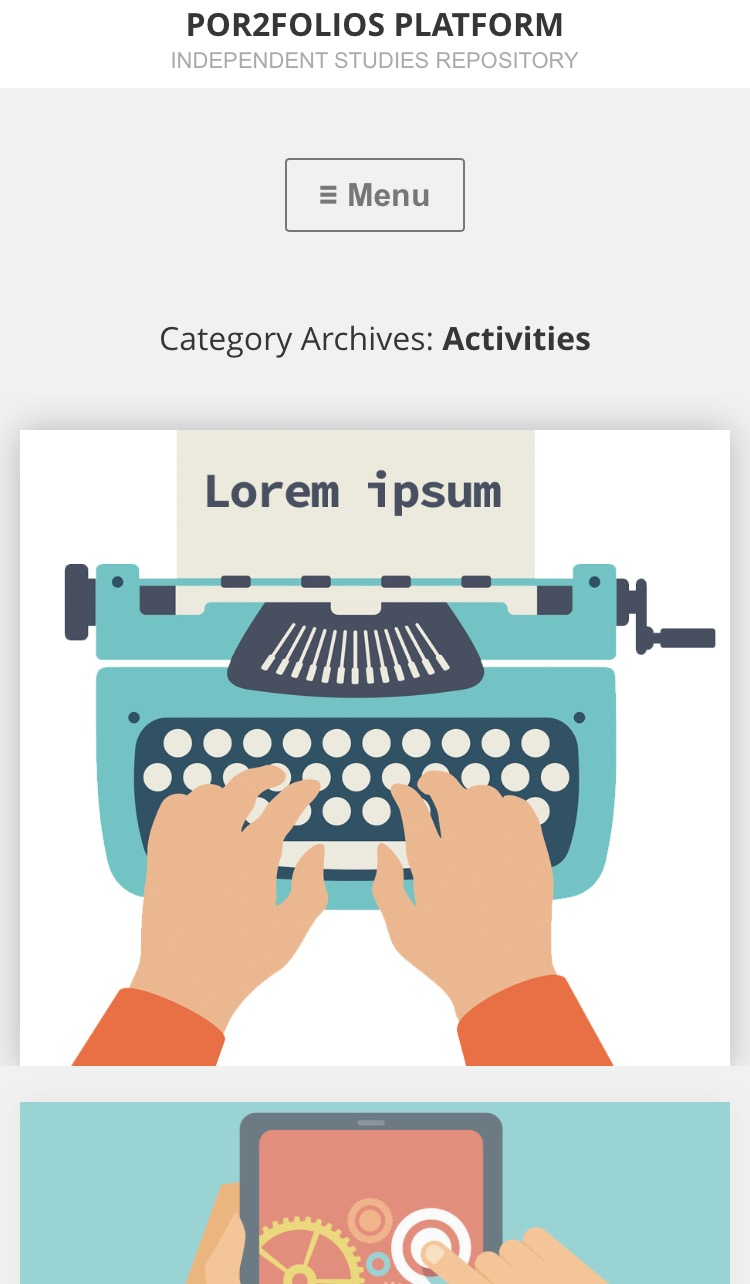
\includegraphics[width=1\linewidth]{mobile.png}
	\caption{The Platform}
	\label{fig_sim}
\end{figure}

\section{The Developed Work} 
After several meetings with the team I was able to understand what the platform requirements were, what had already been developed, what tools were used and what still needed to be done. Integration with the team was a challenging albeit smooth experience. Having no experience with development using \ac{CMS}, more specifically WordPress,  I had to catch up with what was already implemented and how it worked. In doing so I learned the inner workings and requirements of an online platform. After an adaptation period, where my colleagues helped me integrating with the team, I was tasked with the challenge of adding a large number of tags to the platform. This required me to do some research on methods of achieving such a task. The results of my research led me to believe that my task could be achieved in two ways:

\begin{itemize}
	\item A brute force approach -- I could manually add the tags through the WordPress Administrator \ac{GUI}. Doing so required me to add each tag individually, which given the amount of tags to add would be a time consuming task;
	\item A more efficient approach -- Considering that WordPress provides an API for scripting that is vastly documented I could create a PHP script to instantiate the necessary tag entries.
\end{itemize}

Despite having very little experience with PHP, I decided to create the script to add the tags to the database. This would further my PHP knowledge along with giving me experience dealing with APIs. With a lot of research and the valuable help of my colleagues I was able to create the necessary script that iterated through the text file containing all the tags and added them to the WordPress Database. Due to constraints within the API, that does not allow directly adding tags, the script uses a work-around. This helped me develop my improvisation skills as it required me to think outside the box and get creative, having no clear way of adding the necessary tags.  It also required me to get to know the WordPress API which in turn gave me new ideas to further develop the platform.

%%%%%%%%%%%%%%%%%%%%%%%%%%%%%%%%%%%%%%%%%%%%%%%%%%%%%%%%%%%%%%%%%%%%%%%%%%%%%%%%
%%%%%%%%%%%%%%%%%%%%%%%%%%%%%%%%%%%%%%%%%%%%%%%%%%%%%%%%%%%%%%%%%%%%%%%%%%%%%%%%
\section{Learned Skills}
There are several \textit{soft-skills} that an individual should try to develop. They are paramount in the day-to-day interactions with other people and help in achieving cooperation and communication. 

Probably the most important lesson to take away from this experience is to be pro-active. Had I shown such pro-activeness earlier I could have join the development process right at the start. It is of extreme importance to actively look for opportunities and not sit idly waiting for them to come by.

During my activity I was forced out of my comfort zone and had to deal with tools that I had never used before. The help from my colleagues was invaluable in overcoming the difficulties and problems I faced. The work experience was really smooth considering that, as we later discovered, we are all part of \ac{INESC} so working together and meeting regularly was really easy. I improved my communication skills as well as my self-learning and adaptation capabilities. 

The report itself introduced me to a powerful new tool, that will surely be of use in my work/student  life, and allowed me to further develop my English writing skills. 



%%%%%%%%%%%%%%%%%%%%%%%%%%%%%%%%%%%%%%%%%%%%%%%%%%%%%%%%%%%%%%%%%%%%%%%%%%%%%%%%
\section{\IfLanguageName{english}{Conclusion}{Conclusão}}
This experience was definitely valuable for me as a person. I was able to develop new skills as well as improve skills I already had acquired. Even though most of the challenges I faced were technical ones, the ability to communicate and adapt to the situation was paramount to achieve results.  In the future I, along with the rest of the development team, intend to continue working on the Por2Folios platform. I believe the work we did and the platform we developed will be a valuable tool to the future students enrolled in the Portfolio course. As such I will strive to improve the platform as well as further improve my \textit{soft-skills}. 
%%%%%%%%%%%%%%%%%%%%%%%%%%%%%%%%%%%%%%%%%%%%%%%%%%%%%%%%%%%%%%%%%%%%%%%%%%%%%%%%
% use section* for acknowledgement
\ifCLASSOPTIONcompsoc
  % The Computer Society usually uses the plural form
  \section*{\IfLanguageName{english}{Acknowledgments}{Agradecimentos}} % Acknowledgments
\else
  % regular IEEE prefers the singular form
  \section*{Acknowledgment}
\fi

I would like to thank all the people that somehow contributed to my experience. The development team for integrating me and helping me overcome the obstacles I faced. Professor Rui Cruz for being understanding and allowing me to join the development team mid-development as well as doing so quickly and efficiently. Lastly I would like to thank Joana Teixeira, girlfriend and invaluable \LaTeX connoisseur.
%%%%%%%%%%%%%%%%%%%%%%%%%%%%%%%%%%%%%%%%%%%%%%%%%%%%%%%%%%%%%%%%%%%%%%%%%%%%%%%%

%%%%%%%%%%%%%%%%%%%%%%%%%%%%%%%%%%%%%%%%%%%%%%%%%%%%%%%%%%%%%%%%%%%%%%%%%%%%%%%%
% biography section
% 
\begin{IEEEbiography}[{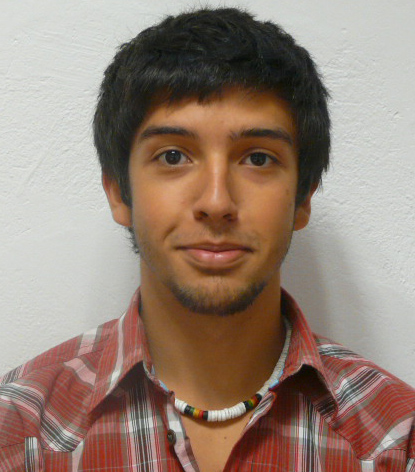
\includegraphics[width=1in,height=1.25in,clip,keepaspectratio]{nuno.png}}]{Nuno Sousa}
Here I am. I am pursuing my Computer Engineering studies at \ac{IST}. I have a special interest in the Computer Graphics area, which my thesis will focus on. I love Photography and I pursuit it as one of my hobbies.
\end{IEEEbiography}

%%%%%%%%%%%%%%%%%%%%%%%%%%%%%%%%%%%%%%%%%%%%%%%%%%%%%%%%%%%%%%%%%%%%%%%%%%%%%%%%
\newpage
\onecolumn
%%%%%%%%%%%%%%%%%%%%%%%%%%%%%%%%%%%%%%%%%%%%%%%%%%%%%%%%%%%%%%%%%%%%%%%%%%%%%%%%
%%%%%%%%%%%%%%%%%%%%%%%%%%%%%%%%%%%%%%%%%%%%%%%%%%%%%%%%%%%%%%%%%%%%%%%%%%%%%%%%
% *** DEFINITION OF ACRONYMS ***

	
	
	
% that's all folks
\end{document}